
%pp.~150--153

\chapter{Convolutional neural networks}
\label{convolutional_neural_networks}

This chapter introduces convolutional neural networks, also known as convnets. There exist different types that can be used for various tasks. While one dimensional convolutional neural networks (1D convnets) can be used for sequence classifications \cite[Chapter~6]{cnn}, two dimensional convolutional neural networks (2D convnets) are almost universally used in the area of computer vision \cite[Chapter~5]{cnn}. There are other types of convnets, but this work utilizes only those two. Therefore, only they will be explained. Furthermore, only the concepts relevant for this work will be covered. To explain the concepts of convnets, 2D convnets will we used. Once understood, they can easily be applied to 1D convnets, as there is little difference between the two types of models. The differences that exist, will be explained. 

Convnets consist of multiple components called layers \cite[Chapter~3]{cnn}. Which combination of layers to use is highly dependent on the data and its complexity. Same goes for the choice of the so-called hyper parameters. These parameters play a major role in how the model is trained and how it will perform. Two important hyper parameters are the number of epochs and the learning rate \cite[Chapter~4]{hyper}. While the number of epochs describes how often the whole training data should be passed to the network, the learning rate controls how much the network adapts to the training data in each epoch. How neural networks are trained is explained in chapter \ref{training_neural_networks} \nameref{training_neural_networks}. More specific to convnets are the parameters for the size of the patches extracted from the inputs and the depth of the output feature map \cite[Chapter~5]{cnn}, described in section \ref{convolution_layers} \nameref{convolution_layers}. Finding the best hyper parameters to optimize the network can be done in various ways, for instance using evolutionary algorithms \cite{evolution}. However, this is not part of this work. 

\newpage

\section{Layers}
\label{layers}
The convolutional neural networks used in this work consists of the following types of layers: convolution layers, dense layers, also known as densely connected layers, dropout layers, pooling layers and flatten layers. They will be explained without going too much into detail about the exact calculations performed.

\subsection{Convolution layers}
\label{convolution_layers}
Convolutions operate over three dimensional tensors and are defined by two key parameters: The size of the windows that extract patches from the inputs and the depth of the output feature map. Typically the size of these windows is 3 x 3 or 5 x 5. The depth of the output feature map can also be interpreted as the number of filters computed by the convolution. A convolution is performed by moving these two dimensional windows step by step across the three dimensional input feature map and extracting a three dimensional patch of surrounding features in each step. Each resulting patch has the height and width of the window and the depth of the input feature map \cite[Chapter~5]{cnn}. Figure \ref{fig:loc} exemplary shows the valid locations of 3 x 3 windows in a three dimensional input feature map with a height and width of 5 and an arbitrary depth.


%Convolutions operate over three dimensional tensors and are defined by two key parameters: The size of the patches extracted from the inputs and the depth of the output feature map. Typically the height and width of these patches is 3 x 3 or 5 x 5 and the depth is that of the input feature map. The depth of the output feature map can also be interpreted as the number of filters computed by the convolution. A convolution is performed by moving two dimensional windows step by step across the three dimensional input feature map and extracting a three dimensional patch of surrounding features in each step. Figure \todo{ref} exemplary shows the valid locations of 3 x 3 patches in an 5 x 5 input feature map.

\begin{figure}[H]
	\centering
	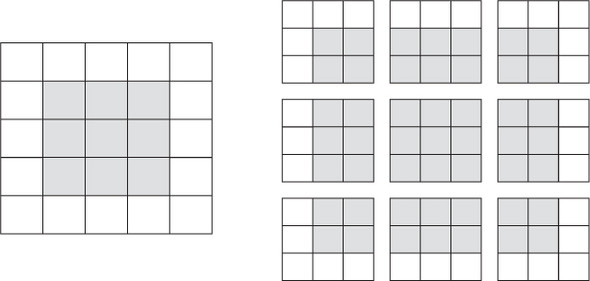
\includegraphics[width=10cm]{images/nn/loc.jpg}
	\caption[Valid locations of 3 x 3 windows in a feature map.]{Valid locations of 3 x 3 windows in a feature map with arbitrary depth and a height of 5 x 5. Top view fn the feature map. The depth is not shown.  Source: \cite[Chapter~5]{cnn}.}
	\label{fig:loc}
\end{figure}

Afterwards, each of these three dimensional patches is transformed into a one dimensional vector that has the specified depth of the output feature map. This transformation is done by calculating a tensor product with a weight matrix, called the convolutional kernel. The kernel has the same dimensions as the window that extracts the patches. The weights of the convolutional kernel are randomly initialized and learned during the training of the network. Once a vector for each patch is calculated they are combined into a three dimensional output feature map. This is done in a way so that every spatial location in the output feature map correspond to the same location in the input feature map \cite[Chapter~5]{cnn}. The whole process of a convolution is shown in figure \ref{fig:conv}.

\begin{figure}[H]
	\centering
	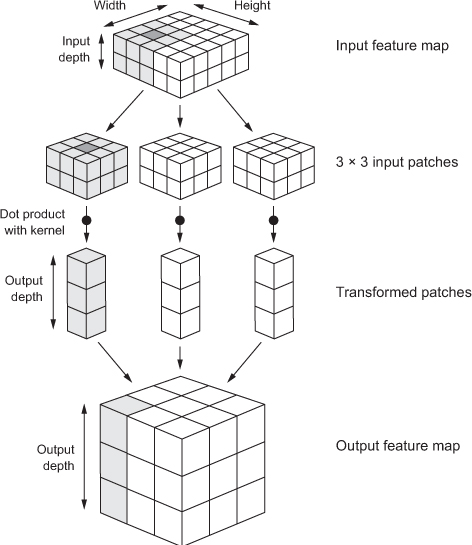
\includegraphics[width=10cm]{images/nn/conv.jpg}
	\caption[The whole process of a two dimensional convolution.]{The whole process of a two dimensional \\convolution. Source: \cite[Chapter~5]{cnn}.}
	\label{fig:conv}
\end{figure}

The way the convolution is performed is also what makes convolution layers fundamentally different from densely connected layers that are explained in section \ref{dense} \nameref{dense}. Dense layers learn global pattern in their input feature space, while convolution layers learn local patterns. These local patterns are found in the patches of specified size extracted from the input. This characteristic gives convolutional neural networks two important properties. First of all the patterns they learn are translation invariant, meaning that for instance after learning a pattern in the lower left corner of an image it can be recognized anywhere in the image. Contrary to that densely connected networks would have to learn the pattern new if it appeared in a different location on the image. The second characteristic is that convolutional neural networks can learn spatial hierarchies of patterns. The first convolution layer can learn small local patters like edges and the next convolution layer will receive the features of the first layer and learn larger patterns, and so on, resulting in the ability to learn increasingly complex patterns \cite[Chapter~5]{cnn}.

Last but not least it should be mentioned that the 3D input tensor of such a convolution layer can be created from an image, where the height an the width of the image are that of the tensor and the different colour channels of the image are represented by the depth of the tensor. However, after an image is passed through a convolution layer a new output feature map is produced and its depth is specified by one of the parameters mentioned above. As a result the depth channels no longer represent the different colour channels of the input image. Instead they are referred to as filters, that encode specific aspects of the input data \cite[Chapter~5]{cnn}. 

\subsection{Max-Pooling layers} 
\label{max_pooling}
There are multiple types of pooling layers, but max-pooling is the only pooling operation used in this work as is tends to work better than the alternative solutions \cite[Chapter~5]{cnn}. Pooling operations are generally used to downsample the feature maps. Max pooling is performed by extracting windows, usually the size of 2 x 2, from the input feature map and outputting the highest value of each channel. Such a window size halves the height and width of the feature map. This aggressive downsampling has two effects. Firstly, the computational complexity is reduced massively as their are less values to process and secondly, it has as result that the data in the patches extracted from the inputs in successive convolution layers contain information about increasingly larger areas of the original input image. Therefore, the size of the region in the input data that has influence on the individual features created by the convolution is increased \cite[Chapter~5]{cnn}. This increase is a fundamental concept of convolutional neural networks and is further explained in section \ref{receptive_field} \nameref{receptive_field}.


\subsection{Dropout layers}
\label{dropout}
The overall aim is to create models that generalize, meaning they perform well on data that they have never seen before. The central obstacle of generalization is overfitting. It describes the scenario in which the model adapts to much to the training data which reduced its ability to generalize. An effective way to reduce overfitting is using a dropout layer. Dropout is a technique originally developed by Geoff Hinton and his students at the University of Toronto \cite{hinton}. It is applied to a layer by randomly setting a number of output features of the layer during training to 0. The rate in which this happens can be specified and is usually between 0.2 and 0.5. In short, the idea is, that randomly setting output to 0 produces noise that can break up random patterns which are not significant and otherwise would be memorized by the model if no noise was present \cite[Chapter~4]{cnn}. 

\subsection{Flatten layers}
\label{flatten}
A flatten layer simply receives a multi dimensional input tensor, in case of 2D convnets this tensor is three dimensional, and flattens it into a 1D tensor that can be fed to a densely connected network \cite[Chapter~5]{cnn}. 

\subsection{Dense Layers}
\label{dense}
After flattening, the resulting 1D tensor is generally passed to a densely connected network \cite[Chapter~5]{cnn}. This network consists of multiple dense layers that classify the input features. In dense layers each feature depends on the whole of the input data. Each layer applies tensor operations, that involve weights randomly initialized and learned during the training of the network. The final layer in a classification task often is a dense layer with softmax activation that returns an array in the size of the number of classes, specifying probabilities for each class \cite[Chapter~2]{cnn}. Activation functions are briefly explained in section \ref{activation} \nameref{activation}. 

\newpage

\section{Activation functions} 
\label{activation}
In this work, activation functions are used in combination with convolution and dense layers. One activation function, the softmax function, has been already mentioned in section \ref{dense} \nameref{dense}. It produces an array that implies the prediction of the model. In short, activation functions simply receive an input and calculate an output depending on that function. The other activation function that is utilized in this work is the rectified linear unit (relu). It enables the the layer to learn non-linear transformations of the input data. In comparison to otherwise being limited to linear transformations this gives the model access to a much richer hypothesis space. All the relu does is take the input and return 0 if the input in less than 0 and otherwise return the input value \cite[Chapter~3]{cnn}. For instance, if combined with a convolution layer, each value in the output feature map is passed to the relu. This results in a new feature map that is passed to the next layer. 

%Each data point can be seen as seen as artificial neuron and the relu, if used, decides which of these neurons fires, meaning which data is set to 0 and which reaches the next layer. In convolution layers for instance each cell of a feature map can be understood as such an artificial neuron. As the the name implies, this concept was inspired by how human neurons operate. Artificial neural networks were invented in an attempt to build artificial systems based on computational principles used by nervous system \todo{ref}. However, this does not mean that they function like human brains. In fact, there are many differences between artifial neural networks an brains. bla highlights this by comparing artificial neural networks trained to classify images with newborn children. An exemplary artifical neural network requires millions of images for the training. Especially as it is a supervised machine learining algorithm, feedback in the form of labels is necessary regarding whether the classifications of the network were correct. If newborn children were limited to the capabilities of artificial neural networks and the way supervised machine learning algorithms function and assuming they could ask one question every second, it would take a life time for them to learn to categorize objects. 

\section{Receptive field}
\label{receptive_field}
One of the fundamental concepts of convolutional neural networks is the receptive field, or field of view, of a feature in a certain layer of the network \cite[p.~1]{receptive}. As mentioned before, in dense layers the features depend on the whole input, while a feature in a convolution only depends on a local region of the input. This region is the receptive field of that feature. 

\begin{minipage}{0.4\textwidth}
	The receptive field size of features in the network can be increased in multiple ways. One way is by stacking more convolution layers, which increases the receptive field size linearly by theory. This effect is visualized in figure \ref{fig:rec}. Another, more effective way, is to use a pooling layer for subsampling, which increases the receptive field size multiplicatively \cite[p.~1]{receptive}. As a result these methods can be used to increase the region size of the original input image that has influence on individual features in deeper layers. 
\end{minipage}
\begin{minipage}{0.6\textwidth}
	\begin{figure}[H]
		\centering
		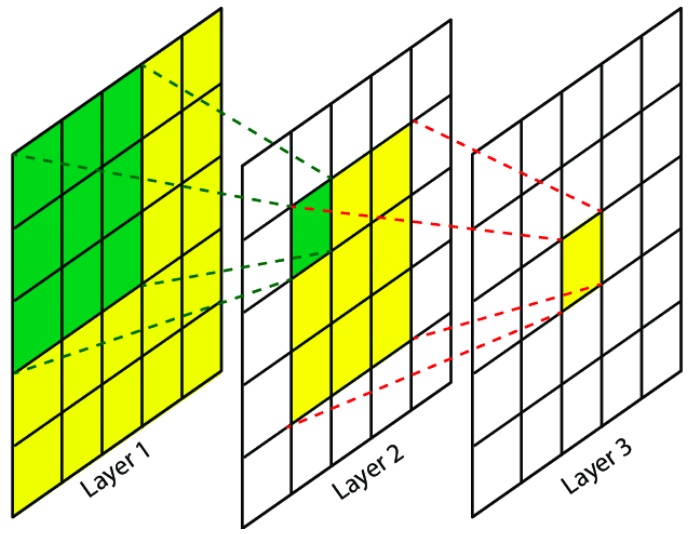
\includegraphics[width=8cm]{images/nn/rec.png}
		\caption[Visualization of a linearly growing receptive field in stacked convolutions.]{Visualization of a linearly growing\\\hspace{0\textwidth} receptive field in stacked convolutions.\\\hspace{0\textwidth} Source: \cite{convIm}.}
		\label{fig:rec}
	\end{figure}
\end{minipage}


These considerations are important when building a model. As stated by Luo et al.: \enquote{Since anywhere in an input image outside the receptive field of a unit does not affect the value of that unit, it is necessary to carefully control the receptive field, to ensure that it covers the entire relevant image region} \cite[p.~1]{receptive}. The features are here referred to as units. This means that if there are regions of a certain size in the input image that should influence individual features as a whole, it is important to make sure when constructing the model that the receptive field in deeper layers is large enough for the specific task.

\newpage

\section{Differences of one dimensional \\convolutional neural networks}
\label{differences_1d_2d}
1D convnets can be used to classify sequence data. Instead of a 3D tensor, they receive 2D tensors as inputs. Such sequence data could for instance consist of muscle activity over time and the task could be to classify the type of movement. The convolutions explained in section \ref{convolution_layers} \nameref{convolution_layers} are two dimensional as the window that extracts patches from the image moves in two dimensions. The convolutions in 1D convnets are one dimensional, meaning the windows only move in one dimension and extract local patches from the sequence. Apart from this the convolution is performed similarly \cite[Chapter~6]{cnn}. The process of a one dimensional convolution is shown in figure \ref{fig:conv1d}. 
\begin{figure}[H]
	\centering
	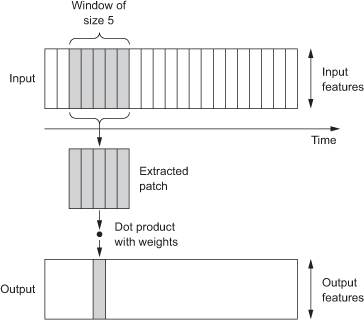
\includegraphics[width=10cm]{images/nn/conv1d.jpg}
	\caption[The whole process of a one dimensional convolution.]{The whole process of a one dimensional convolution. \\Source: \cite[Chapter~6]{cnn}.}
	\label{fig:conv1d}
\end{figure}

The other difference is how the max-pooling operation is performed. Instead of extracting 2D patches and and outputting the maximum value, this is done for 1D patches. The effects of this operation are the same as in 2D convnets \cite[Chaper~6]{cnn}. 

The special characteristics of 2D convnets also apply to 1D convnets. They are translation invariant and capable to learn hierarchical patterns. Furthermore the dropout, flatten and dense layers as well as activations function in the same way. The behaviour explained in section \ref{receptive_field} \nameref{receptive_field} can also be applied to 1D convnets: The patches extracted from the inputs in successive convolution layers contain information about increasingly larger areas of the original input sequence \cite[Chaper~6]{cnn}.

\chapter{Training neural networks}
\label{training_neural_networks}
Although the different components of convnets have been covered in chapter \ref{convolutional_neural_networks} \nameref{convolutional_neural_networks}, it has not been addressed yet, how these networks are trained to make accurate predictions. Therefore, the general concepts involved in training neural networks will be briefly explained.  

\begin{minipage}{0.45\textwidth}
	The relationship between the core concepts revolving around training neural networks is shown in figure \ref{fig:nn_comp}. The fundamental data structure in neural networks is the so called layer. There are many different types of layers that are chained together to form the network. In a classification task, what the network does is map the input data to a prediction. This is also called forward passing, as each layer performs operations on the received data and passes the results to the next layer. Once this chain reaches the output layer and by that outputs a prediction, the loss function takes that prediction as well as the actual target label and calculates a loss value which is a measure of how well the network's predictions match the expected outcome. 
\end{minipage}
\begin{minipage}{0.55\textwidth}
	\begin{figure}[H]
		\centering
		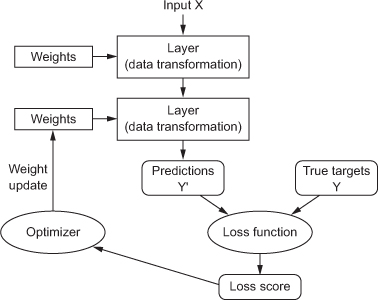
\includegraphics[width=8cm]{images/nn/comp.jpg}
		\caption[Core concepts in training neural networks.]{Core concepts in training\\\hspace{0\textwidth} neural networks. Source: \cite[Chapter~3]{cnn}.}
		\label{fig:nn_comp}
	\end{figure}
\end{minipage}

This value is used by the optimizer to update the networks weights. This is done through an algorithm called backpropagation which works backward from the output layer to the input layer and computes the contribution that each weight had in the loss value. Using a method called stochastic gradient descent, the weights are adjusted in small steps to reduce the loss. The procedure of making predictions, calculating the loss and updating the weights is repeated many times, so that the loss is step by step reduced, resulting in more accurate predictions \cite[Chapter~3]{cnn}.


\begin{comment}
	\chapter{Convolutional neural networks notes}
	As convolutional layers are complex and have many variations for differnet use cases, only concepts and functionaslities that are relevant for this work will be covered. This also menas that 3 dimensional cnns will not be explained, but in generel cnns function the same way whether they have 1, 2 or 3 dimensions. The main differnce lies in how the filter, also known as kernel or festure detector, moves acrross the data. This is later explained in more detail. (\todo{ich glaube input data ist keine regel sondern nur meist so..zum beispiel kann man auch 1d convoltion bei 1d, 2d, oder 3d daten machen}). \\
	First of all the core concepts of cnns will be explained and afterwards the models used in this work will be described.\\
	
	On of the core concepts of convoluntional neural networks are the concolutions. \\
	
	
	
	
	Unituitievly, a 2d cnn must not neccerailty have 2 dimensional data as input.
	
	notes bei models:\\
	- stride = wie viele schritte auf einmal, default 1 deshalb vermute ich bei mir 1\\
	- maxpooling: pool size = 2*2, und bei keras wird stride dann defauklt auch zu 2*2 (=pool size)\\
	- input size = 85*40 glaube ich\\
	- filter weights are randomly initialized, so that they dont all initially learn the same feauters. To briefly explain the behaviour of filters a seperation bettween two cases can be made: The first case is that not all features of high quality have been learned yet, high quality meaning that learning them would lower the cost function. In that case it is highly unlikely that each filter would begin to resemble other filters, as that would most certainly result in an increase of the cost function and therefore no gradient descent algorithm would head in that direction. The other case is that all features of high quality have already been leanred by a subset of the avaibable filters. In this case the cost function would not be increased if the remaining filters learn similar features than the other filters. \\
	- in einem der schritte wird eine zeile usgelassen, aber ich trainiere nicht nochmal alles neu (oder?)\\
	
	- 1d and 2d convolution
	- reduction of dimension
	- relu 
	- number od filter, random initializion, etc
	- kernel and kernel size
	- loss function and optimizer, stochastic gradeint decent
	- Dropout layers
	- Pooling, max pooling 
	- flatten
	- dense relu, softmax
	- droput layer, pooling ändert nichts an der anzahl der fetsure maps
	- \todo{bessere quelle finden, buch oder so}
	- stride (ganz kurz, beschriebt verhalte wenn etwas über bleibt, zero padding oder weglassen)
	- back propagation
	- wie schaffen die es bspw. 64 feature maps auf 32 zu reduzieren? also wie funktionieren die filter in dem fall? 
	- receptive field 
\end{comment}


  


